\documentclass[10pt,twocolumn,letterpaper]{article}

\usepackage{cvpr}
\usepackage{times}
\usepackage{epsfig}
\usepackage{graphicx}
\usepackage{amsmath}
\usepackage{amssymb}
\usepackage{bm}

% Include other packages here, before hyperref.

% If you comment hyperref and then uncomment it, you should delete
% egpaper.aux before re-running latex.  (Or just hit 'q' on the first latex
% run, let it finish, and you should be clear).
%\usepackage[pagebackref=true,breaklinks=true,letterpaper=true,colorlinks,bookmarks=false]{hyperref}

\cvprfinalcopy % *** Uncomment this line for the final submission

\def\cvprPaperID{****} % *** Enter the CVPR Paper ID here
\def\httilde{\mbox{\tt\raisebox{-.5ex}{\symbol{126}}}}

% Pages are numbered in submission mode, and unnumbered in camera-ready
\ifcvprfinal\pagestyle{empty}\fi
\begin{document}

%%%%%%%%% TITLE
\title{W4735 Visual Interfaces to Computers\\Final Project Report: Real-time Gesture-based Game Control}
\author{Jie Huang and Shao-Chuan Wang\\
Department of Computer Science\\
Columbia University\\
{\tt\small \{jh3105, sw2644\}@columbia.edu}
% For a paper whose authors are all at the same institution,
% omit the following lines up until the closing ``}''.
% Additional authors and addresses can be added with ``\and'',
% just like the second author.
% To save space, use either the email address or home page, not both
}

\maketitle
\thispagestyle{empty}

%%%%%%%%% ABSTRACT
\begin{abstract}
In this report, we are going to introduce a system that exploits two bare hands image 
as visual input to control a real-time game. We firstly perform skin segmentation using hue-saturation 
thresholding on colored images. Since faces are also in skin color, we 
use face detection to prune the faces. After obtaining the contours of two 
bare hands, we find the finger tips of hands by finding the top of the contour.
We use a line between two finger tips to control the game; the position of the line 
and its orientation have a mapping to the controlled object. The tools we used are python wrapper 
of OpenCV 2.1 library, and pygame for game development.
\end{abstract}

%%%%%%%%% BODY TEXT

\section{Introduction}

Visual interfaces in the applications of human-computer interface 
have been progressed tremendously in recent years. In particular, an outside-out 
visual system \cite{outout} which does not require players to wear 
any extra devices provides flexibilities in gaming applications, if 
the motion of the body can be accurately captured.
As we can see from the recent example, Microsoft Kinect, is the 
first vision-based commercial game platform, and it does 
create a lot of new paradigms for playing video games with human bodies. 

However, the idea of using gesture or human body as game
controllers appeared in 1990s. For example, 
Freeman et al. \cite{cvicg, cvfcg} implemented a computer vision based 
computer game system, based on image moments and orientation histograms, and 
use the chips to provide real-time interactive responses to the players. 

More recently, H\"{a}m\"{a}l\"{a}inen \cite{childgame} designed a perceptual user interface for
controlling a flying cartoon-animated dragon in a
physically and vocally interactive computer game for 4 to 9 years old children.
Lu et al. \cite{racecar} proposed a vision-based 3D racing car game controlling
method by analyzing the distance of two fists positions of the player
from the camera to control the direction of the racing car. Similarly, 
Schlattmann \cite{3dgames} et al. demonstrated three 3D real-time games via bare-handed 
interactions. All studies show higher usability via vision-based gesture controls 
in their usability tests.


In this proposal, we propose to to build a gesture-based game controller, which 
requires the modern computer vision technology. For a detailed review on visual 
interface of hand gestures and human motion capture, please see 
the review articles \cite{pamireview, cviureview}.

\section{Design decisions}
\subsection{Hardware}
Table~\ref{tab:hw} compares different hardware devices.
Our team considered to use Kinect to implement the system; however, 
we chose to use normal laptop web camera due to its availability as well as its 
low cost. 
Our webcams have frame rates ranging from 15fps to 30fps, which is adequate for real-time 
game control. Also, we need a colored camera in order to detect the skin color.

\begin{table}[h]
\begin{tabular}{c|ccc}
&High-end\\
&Camera&Web Camera&Kinect \\
\hline
Frame rates & fast & adequate & adequate \\
Resolution & HD 1080 & VGA & VGA \\
Availability & medium & high & low \\
Skin detection & not very easy & not very easy & very easy \\
Noises & low & high & medium \\
Cost & high & low & high 
\end{tabular}
\caption{The comparison between different capturing devices.}
\label{tab:hw}
\end{table}

\subsection{Software}
We used python as our development programming language due to 
its dynamic and high-level properties. We use python for rapid 
development. Python has OpenCV wrapper, and hence we can tune 
the parameters quickly without recompiling the whole system. 
Python has a game development package called pygame, which 
has event handling, sound handling, and screen drawing for making 
games. To fulfill the needs to gesture-controlled game development, 
we find python has good library supports and easy for development.

As a brief summary, we chose python as our developing programming 
language due to the following reasons:
\begin{itemize}
	\item Python is cross-platform. We are developing on Mac OS and Windows simultaneously.
	\item Python is dynamic and high-level. Good for rapid development.
	\item Python is an interpreter. We don't need to recompile the codes as we are trying some parameters.
	\item Python has abundant library support such as OpenCV and pygame. 
\end{itemize}

In this project, we are focusing on the visual interface 
design. Hence, we do not intend to build a game from the scratch. 
Instead, we chose to modify an exisiting game which is open sourced. 
The original version of pybreakout can be downloaded at
\verb"http://code.google.com/p/pybreakout/"

\subsection{Game: breakout}
We choose an ancient Nintendo game \emph{Breakout} and modify 
the control of the paddle. Traditionally, the paddle can 
move only horizontally along a predetermined line at a constant speed.
In our design, we choose to enable the paddle to move upward and rotate.
The reason why the traditional design may be the reason that 
it is not intuitive to rotate the paddle with gamestick.
\begin{figure}[h]
\centering
\begin{tabular}{cc}
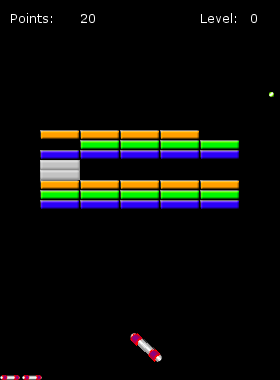
\includegraphics[height=3.5cm]{game0060.png} &
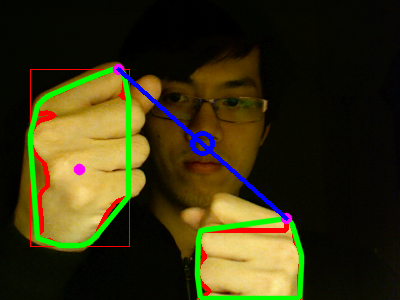
\includegraphics[height=3.5cm]{gesture0060.png} \\
(a) Game play screen &
(b) Control screen
\end{tabular}
\caption{A screenshot of playing \emph{breakout}}
\label{fig:gamescreen}
\end{figure}

However, if we control the orientation and position of the paddle 
using the gesture shown in Figure~\ref{fig:gamescreen} (b), 
we can control the paddle according to our gesture commands.

Figure~\ref{fig:gamescreen} (b) shows our design of control. 
We use tips of two bare hands as references, and the orientation and 
the position of the paddle is controoled by the blue line in 
Figure~\ref{fig:gamescreen} (b).

We can also easily extend this controlling interface to other 
games such as car driving games due to the fact that in most 
car driving games, we only need to control the wheel by 
orientation. It would be also very intuitive to control 
the virtual car using two bare hands, as shown in Figure~\ref{fig:cargame}.
\begin{figure}[h]
\centering
\begin{tabular}{cc}
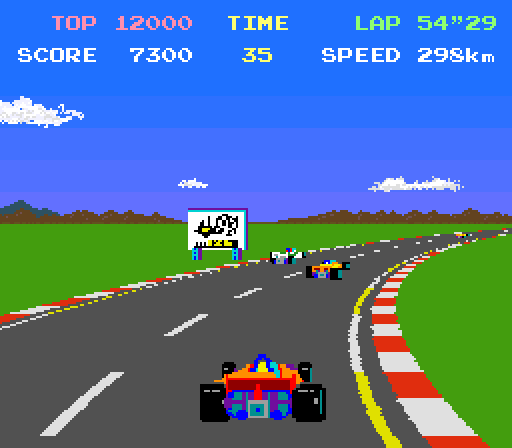
\includegraphics[height=3cm]{cargame.png} &
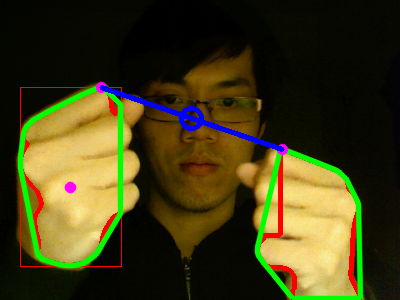
\includegraphics[height=3cm]{gesture0047.png} \\
(a) A car game screen &
(b) Control screen
\end{tabular}
\caption{A concept screenshot of playing a car game.}
\label{fig:cargame}
\end{figure}

\subsection{Machine-human interface: Bare hands}
We chose to use bare hands as our machine-human interface 
to control the game play due to the following reasons:

\begin{itemize}
	\item It is too cubersome to wear any extra devices/markers.
	\item We can extend our work of assignment one.
	\item It is more intuitive to use your own hands to control the game.
	\item You do not have to find and setup the devices before you play.
\end{itemize}

However, it also have disadvantages, and to name a few,
\begin{itemize}
	\item Skin segmentation is not robust.
	\item Images from the webcamera is mostly noisy.
	\item The environment becomes rather restricted. We cannot play in all kinds of environments.
\end{itemize}
To compensate the environment issues, we designed an user-interface 
to adjust the parameters to adapt to different lighting environment as shown in Figure~\ref{fig:adjusting}. 

\begin{figure}[h]
\centering
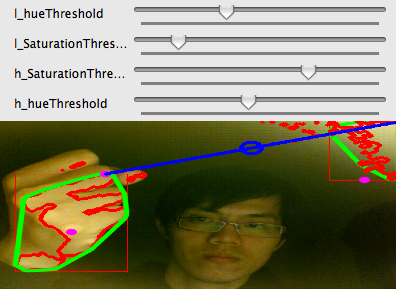
\includegraphics[width=7cm]{adjustui.png}
\caption{A screenshot on the user interface to adjust parameters. We provide 
sliders to adjust system parameters.}
\label{fig:adjusting}
\end{figure}

More details on skin detection will be explored in the next section.

\section{Gesture controller}
\subsection{System overview}
(block diagrams) and how visual interface invoke the movement.

\subsection{Skin detection}

\subsection{Motion detection}

\subsection{Contour finding}
\label{sec:contour}

\subsection{Face pruning}
\label{sec:face}
We described how we use hue and saturation thresholding to detect skin
 color and therefore find the hands; however, faces are also in skin color. 
 The user's face becomes a noise as we interpret the found skin mask as 
 two hands. We may assume that faces are bigger than hands and use 
 the area of found contours to filter out the faces. However, this criterion is not robust. 

 Hence, we chose to use OpenCV builtin face detection to find the faces 
 and wipe it out on the skin mask.

\subsection{Controller algorithms}

\section{Alternative designs of interface}
% rectangle in the center.
% not bare hands

\section{Game perspectives}

\section{System optimization}
% resize
% cache (e.g. face training data)
% game tick vs control tick
A game control interface has to be real-time. In other words, 
the gesture decision has to be made in a very short period of time. 
We faced efficiency issues as we integrate the visual interface and 
the game. We found several ways to optimize the systems without 
sacrifacing the control accuracy.

\paragraph{Resize visual input.} The resolution of 
original visual input image is $640 \times 480$. 
We resize it to $400 \times 300$, and the speed boosted.
We do not need high-resoluted image because we detected 
blobs and contours which do not highly depend on image resolution. 
(the details of detecting the hands are depicted in Section 
\ref{sec:contour}.

\paragraph{Cache.} We do not calculat everything on the fly. 
If something can be done offline, we will precompute it and 
load it as the system starts. For example, in Section 
\ref{sec:face} we filtered out faces by face detection. 
The training face data are loaded only once at the beginning. 
In this way, we reduced the I/O overheads. We also did the 
similar cache for other resources.

\paragraph{Drop frames.} The computation of visual input 
and processing is heavier than the game; To smoothen the game 
play, we drop frames of visual input. We do not ask 
the visual interface to invoke the movement events. 
Hence, we sacrifaced the response time of the visual control 
without sacrifacing the frame rates of the game. In our 
current implementation, the ratio of the frame rates between 
visual control and game is $1/4$.

\section{System limitation}

\subsection{Noisy skin detection results}

\subsection{Control usability}

\section{Conclusion and future direction}
Our visual controlling interface can be applied to other games, 
such as car racing games. Our system have relatively stable control on 
orientation of two hands, and the orientational inforamtion can be 
used to control the direction of the racing car.

{\small
\bibliographystyle{ieee}
\bibliography{egbib}
}

\end{document}
